%%%%%%%%%%%%%%%%%%%%%%%%%%%%%%%%%%%%%%%%%%%%%%%%%%%%%%%%%%%%%%%%%%
%%  ~ Trabajo de Fin de Grado - Universidad de Vigo (ESEI) ~    %%
%% Autor: Diego Enrique Fontán Lorenzo                          %%
%% Tutor: Miguel Ramón Díaz-Cacho Medina                        %%
%% Convocatoria: Julio 2020/21                                  %%
%% Título: Framework de automatización de auditorías Red Team   %%
%%%%%%%%%%%%%%%%%%%%%%%%%%%%%%%%%%%%%%%%%%%%%%%%%%%%%%%%%%%%%%%%%%

%%%%%%%%%%%%%%%%%%%%%%%%%%%%%
%% Data
%%%%%%%%%%%%%%%%%%%%%%%%%%%%%

\chapter{Gestión de los datos e información} \label{cap:data}

En este capítulo se detalla cómo se gestiona la información que maneja la aplicación. El tratamiento de estos datos se realiza de dos maneras diferentes, dependiendo de si son parte del flujo de datos perteneciente a los nodos del editor o a la \textit{API}.\n

%%%%%%%%%%%%%%%%%%%%%%%%%%%%%
%% Nodes
%%%%%%%%%%%%%%%%%%%%%%%%%%%%%

\section{Información de los nodos} \label{sec:nodedata}

Los nodos tienen tres vías principales (las entradas, las salidas y los controles) \fig{nodeskel} y una secundaria (llamadas a la \textit{API}) por las que manejan datos. Las \textbf{entradas} son la información que recibe de otros nodos; \textbf{los controles}, la información que condiciona el comportamiento del nodo y \textbf{las salidas}, la información que transmite en relación a sus entradas y/o controles. Un nodo puede estar formado por cualquier combinación de entradas, salidas y controles.\sn

\begin{figure}[H]
    \centering
    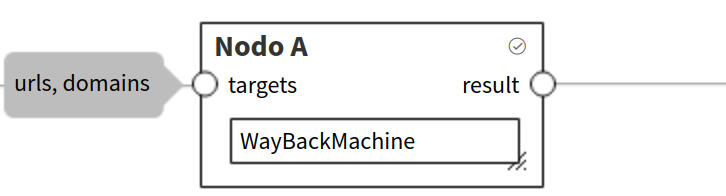
\includegraphics[width=8cm]{img/tables/26_Ingredient.png}
    \caption{Representación de un nodo.}
    \label{fig:nodeskel}
\end{figure}

Las entradas y las salidas se visualizan a modo de conectores (de izquierda a derecha, respectivamente) Las salidas pueden conectarse a las entradas mediante cables y todos los datos que se transmiten están sujetos a un modelo \textit{tipado}, similar a los tipos de variables en los lenguajes de programación tradicionales. Dos conectores con tipos de datos incompatibles no se pueden unir entre sí.\sn

Dichos tipos de datos se generan automáticamente a la par que los nodos, los cuales son especificados mediante un archivo con formato \textit{YAML\footnote{\textit{YAML Ain't Markup Language}. \url{https://yaml.org/}}\fig{ingredientspec}}. Los tipos de datos pueden comprobarse estacionando el cursor encima del conector en el que se esté interesado. Además, existe un tipo de dato, \textbf{\textit{any}}, que no tiene restricciones de conexión.\sn

Respecto a la ejecución, los nodos reportan su estado mediante un icono en la parte superior derecha.

Por otra parte, actualmente existen cuatro estilos de controles diferentes que se pueden implementar en un nodo. Los controles no son más que la abstracción de los elementos propios de formularios \textit{HTML}: \textbf{\textit{Area}}, \textbf{\textit{Check}}, \textbf{\textit{Input}} y \textbf{\textit{Options.}}\sn

\begin{figure}[H]
    \centering
    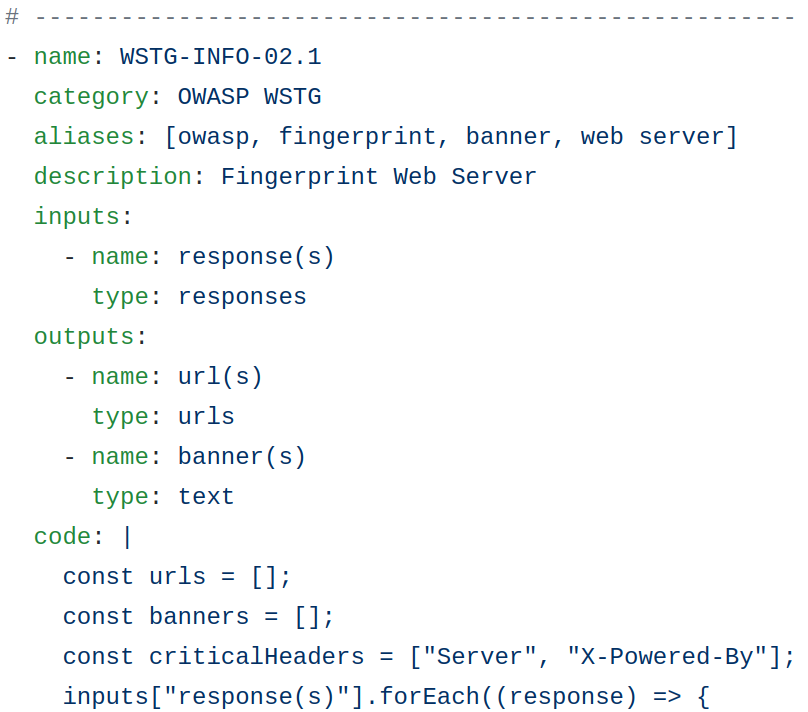
\includegraphics[width=8cm]{img/tables/27_Ingredient-Spec.png}
    \caption{Especificación de un nodo.}
    \label{fig:ingredientspec}
\end{figure}

Por último, tal como se puede observar en la figura \ref{fig:ingredientspec}, los nodos procesan los datos mediante código \textit{JavaScript}. Este código consta de cuatro variables globales principales a la hora de manejar los datos que son: \textit{inputs} (datos de entrada), \textit{outputs} (datos de salida), \textit{node.data} (parámetros de los controles) y \textit{call} (llamadas a la \textit{API} usando \textit{fetch}). Para más información, consultar en el Anexo \ref{anx:manual}.\sn

Además, para evitar bucles infinitos de procesamiento o ejecuciones innecesarias, el motor que maneja el flujo de datos comprueba si los \textit{inputs} o controles han cambiado desde la última ejecución, las entradas requeridas están conectadas y si los datos que se transmiten por ellas son válidos, evitando evaluar el código si alguna de estas condiciones no se cumple.\n

%%%%%%%%%%%%%%%%%%%%%%%%%%%%%
%% API
%%%%%%%%%%%%%%%%%%%%%%%%%%%%%

\section{Información de la \textit{API}} \label{sec:apidata}

Respecto a los datos que maneja la \textit{API} (documentado en profundidad en el Anexo \ref{anx:manual}), viajan a través del protocolo \textit{HTTP}. Al ser un servicio, se pueden realizar peticiones sin necesidad de usar el editor, lo cual permite integrar la \textit{API} en flujos de trabajos externos.\sn

Tal como se explica en el apartado \ref{sec:classdiagram}, cuando llega una petición a la \textit{API}, lo primero que hace es comprobar que tenga el formato correcto. Entre otras cosas, busca dentro de la petición la cabecera personalizada ``\textit{X-Powered-By: Masterchef!}'' y exige que la petición sea realizada usando el verbo \textit{POST}. Posteriormente, procesa los datos en el cuerpo de la petición y envía una respuesta, ambos en formato \textit{JSON}.